\addcontentsline{toc}{section}{Strange Bounce (4)}
\section*{Strange Bounce}

\subsection*{Problem}

\begin{wrapfigure}{r}{\textwidth / 4}
    \centering
    \vspace{-.75cm}
    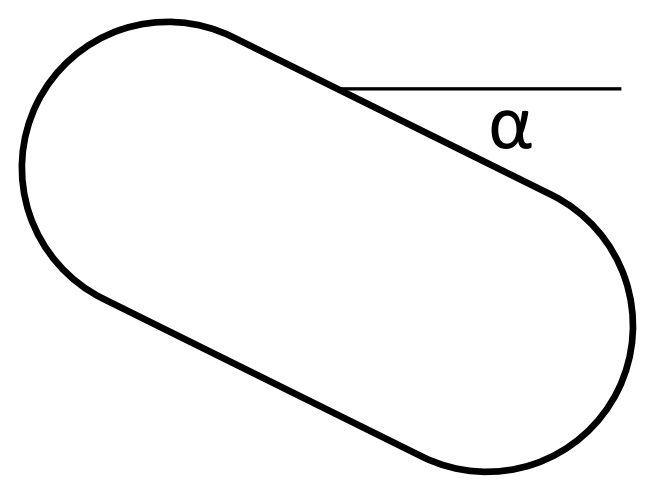
\includegraphics[width = \textwidth / 4]{P-1}
    \caption{}
    \labelf{P-1}
    \vspace{-1cm}
\end{wrapfigure}
The solid object depicted in \reff{P-1} is a cylinder of length
that is $\varepsilon$ times longer then its radius,
with spherical caps on both sides.
Collision\underline{s} of the object with the floor are perfectly elastic.

\begin{enumerate}
    
\item What will be the height ratio to which the object will return
after being dropped from a very big height with orientation $\alpha=0.000$
in cases

\begin{inparaenum}[a)]
    \item $\varepsilon = 0.500$
    \quad \item $\varepsilon = 0.600$
    \quad \item $\varepsilon = 1.500$
    \quad \item $\varepsilon = 1.600$
    \quad \item $\varepsilon = \infty$
\end{inparaenum}

\item For a given value of $\varepsilon$,
    what should be the value of $\alpha$,
    so that the object returns to the same height
    (show one such value of $\alpha$ except $\pm \pi/2$)?
\end{enumerate}

\subsection*{Solution}

The first question that arises, is where can the energy be lost,
so that the object returns to a different height?
The answer is: rotation.
No matter how close $\alpha$ is to $0$,
one side (left or right) of the object reaches the floor earlier than the other.
This off-center collision results in rotation.
The generated rotation can result in yet another collision on the other side.
Multiple consequent collisions may occur this way.

{\bfseries
\begin{enumerate}
    \setcounter{enumi}{-1}
    \item Moment of inertia
\end{enumerate}
}

To calculate the collisions, we first need expression for
moment of inertia of the object with respect to the axis,
around which the rotations will occur.
That axis passes through object's center and is perpendicular to \reff{P-1}'s plane.
There are two types of contributions to the moment of inertia:
the central cylindrical part, and the spherical caps.

The contribution of the cylindrical part is given as an integral over
infinitesimal disks. Disks moment of inertia around its symmetry axis
is known to be $I_d^z=mR^2/2$, where $R$ is the radius and
$m$ is the mass of the disk.
The moment of inertia around a perpendicular axis can be found using
infamous relation $2I^o = I^x + I^y + I^z$,
where $I^o$ is $\int r^2 \differential m$.
For a flat object like the disk $I_d^o = I_d^z$,
and form symmetry we know $I_d^x = I_d^y$. Thus $I_d^x=mR^2/4$.

Using parallel axis (Steiner's) theorem, now we can write the expression
for cylinder's moment of inertia, and evaluate the corresponding integral.
\begin{equation}
    I_c^x = \int\limits_{z=-\varepsilon R/2}^{\varepsilon R/2}
        \differential z \cdot \rho \pi R^2 \inb({\frac{R^2}{4} + z^2})=
        \rho \pi R^5 \inb({\frac{1}{4}\varepsilon+\frac{1}{12}\varepsilon^3})
\end{equation}

Contributions of spherical parts seem easier to calculate.
Moment of inertia of a solid sphere is given by $I_s = 2mR^2/5$,
so semi-sphere's moment of inertia around it's center is also
$I_{ss,o}^x=2mR^2/5$. However parallel axis theorem is applicable only for
moving the axis to or from the center of mass, which is not the semi-sphere center.
Its distance $z_{c,ss}$ from semi-sphere's center can be found as

\begin{equation}
    z_{c,ss} =
    \int\limits_{z=0}^{R}\differential z \cdot z \inb({R^2 - z^2}) \bigg/
    \int\limits_{z=0}^{R}\differential z \cdot \inb({R^2 - z^2}) = \frac{3}{8}R
\end{equation}

Then the semi-sphere's moment of inertia around the object's center is
\begin{equation}
    I_{ss}^x = \frac{2\pi}{3}\rho R^3 \inb({\frac{2}{5}R^2 - z_{c,ss}^2
    + (\varepsilon R / 2 + z_{c,ss})^2}) = \rho \pi R^5
    \inb({\frac{4}{15}+\frac{1}{4}\varepsilon+\frac{1}{6}\varepsilon^2}) 
\end{equation}
which brings the final expression for total moment of inertia to
\begin{equation}
    I^x = I_c^x + 2 I_{ss}^x = \rho \pi R^5
    \inb({\frac{8}{15} + \frac{3}{4}\varepsilon
        + \frac{1}{3}\varepsilon^2 + \frac{1}{12}\varepsilon^3 })
    \equiv \rho \pi R^5 f^{-1}
\end{equation}

The mass is given by
\begin{equation}
    m = \rho \pi R^3 \inb({\frac{4}{3} + \varepsilon}) \equiv \rho \pi R^3 k^{-1}
\end{equation}

{\bfseries
\begin{enumerate}
    \setcounter{enumi}{0}
    \item Collisions
\end{enumerate}
}

Without breaking generality, lets assume the right side collided first ($\alpha>0$).
Consider a collision at arbitrary orientation $\alpha$.
A force is exerted on the bottommost point
(it's the rightmost point of the cylinder in case $\alpha \approx 0$),
which changes both regular and angular momenta of the object.
If velocity before collision is $V$ (upwards),
angular velocity is $\omega$ (clockwise),
and the force momentum is $p$ (upwards), then after the collision
\begin{equation}
    V \rightarrow V + \frac{p k} {\rho \pi R^3} \quad,\quad
    \omega \rightarrow \omega - \frac{p \varepsilon R f \cos\alpha} {\rho \pi R^5}
\end{equation}
After introducing notations $\Omega = \omega \varepsilon R$ and
$P=p/\rho\pi R^3$ for convenience, we can write energy conservation:
\begin{equation}
    \frac{mV^2}{2}+\frac{I\omega^2}{2}=\text{const} \Leftrightarrow
    \frac{V^2}{f}+\frac{\Omega^2}{k \varepsilon^2}  = 
    \frac{(V+Pk)^2}{f}+\frac{(\Omega-Pf\cos\alpha)^2}{k \varepsilon^2}
\end{equation}
from where $P$ can be found to be
\begin{equation}
    P=-2\frac{V-\Omega\cos\alpha}{k+f\cos^2\alpha\varepsilon^2}
    \labele{E-1}
\end{equation}
Afterwards recurrent formulae for $V$ and $\Omega$.
The fact whether the next collision will occur on the right or on the left 
solely depends on the sign of $\Omega$.
As we want to be able to continuously use our right side formulae,
once $\Omega$ becomes negative (next collision is expected on the left),
we will switch and look from the other side, thus changing the sign of $\Omega$.
The recurrent formulae (including the above-mentioned procedure) in case $\alpha=0$ will be
\begin{equation}
    V'=V-(V-\Omega)\frac{2}{1+f\varepsilon^2/k} \quad,\quad
    \Omega'=\inb|{\Omega+(V-\Omega)\frac{2}{1+k/f\varepsilon^2}}|
\end{equation}
Coefficients in the formulae can be calculated in advance for each $\varepsilon$.
\begin{center}
\begin{tabular}{c|c|c|c|c}
    $\varepsilon$ & $k$ & $f$ &
    \(\displaystyle \frac{2}{1+f\varepsilon^2/k} \) &
    \(\displaystyle \frac{2}{1+k/f\varepsilon^2} \) \\
    \hline
    $0.500$ & $0.5455$ & $0.9979$ & $1.3723$ & $0.6277$ \\
    $0.600$ & $0.5172$ & $0.8918$ & $1.2340$ & $0.7660$ \\
    $1.500$ & $0.3529$ & $0.3718$ & $0.5934$ & $1.4066$ \\
    $1.600$ & $0.3409$ & $0.3415$ & $0.5611$ & $1.4389$ \\
    $\infty$ & - & - & $0.1538$ & $1.8462$
\end{tabular}
\end{center}
If counting in terms of initial absolute velocity $V_0$, initially
$(V,\Omega)=(-1,0)$. The question is, when the collisions stop?

Downwards velocity component of the right-bottommost point
(the one, that is going to collide) of the cylinder is $\Omega/2 - V$.
This means, as long as $\Omega > 2V$ immediate collision (with $\alpha=0$) will follow.
But there is also another possibility: no immediate collision occurs
($\Omega < 2V$),
instead some point on the spherical cap hits the floor after some time
(this seems possible, as those points are farther away from the center
and thus have higher rotation velocities).
But it's not possible, as this will require the center of the cap
to be at height $R$, which is not possible, as it's moving upwards.

Now we just have to plug the numbers into recurrent relations,
until there are no more immediate collisions.
Then return height ratio is given by $(V/V_0)^2$.
\begin{center}
\begin{tabular}{c|cc|cc|cc|cc|cc}
    $\varepsilon$ &
    \multicolumn{2}{c|}{$0.500$} &
    \multicolumn{2}{c|}{$0.600$} &
    \multicolumn{2}{c|}{$1.500$} &
    \multicolumn{2}{c|}{$1.600$} &
    \multicolumn{2}{c}{$\infty$}\\
    \hline
    $N$ & $V$ & $\Omega$ & $V$ & $\Omega$ & $V$ & $\Omega$ & $V$ & $\Omega$ & $V$ & $\Omega$ \\
    \hline
    0 & -1     & 0      & -1     & 0      & -1      & 0      & -1      & 0      & -1      & 0    \\
    1 & 0.3723 & 0.6277 & 0.2340 & 0.7660 & -0.4066 & 1.4066 & -0.4389 & 1.4389 & -0.8462 & 1.8462 \\
    2 &        &        & 0.8904 & 0.3585 & 0.6694  & 1.1437 & 0.6147  & 1.2632 & -0.4320 & 3.1243 \\
    3 &        &        &        &        &         &        & 0.9785  & 0.3300 &  0.1152 & 3.4411 \\
    4 &        &        &        &        &         &        &         &        &  0.6268 & 2.6991 \\
    5 &        &        &        &        &         &        &         &        &  0.9456 & 1.1266 \\
    6 &        &        &        &        &         &        &         &        &         &        \\
    \hline
    $h/h_0$ &
    \multicolumn{2}{c|}{$0.139$} &
    \multicolumn{2}{c|}{$0.793$} &
    \multicolumn{2}{c|}{$0.448$} &
    \multicolumn{2}{c|}{$0.956$} &
    \multicolumn{2}{c}{$0.894$}\\
    \hline
\end{tabular}
\end{center}

{\bfseries
\begin{enumerate}
    \setcounter{enumi}{1}
    \item Same height jump
\end{enumerate}
}

The energy conservation low has two (entwined) solutions.
One of the solutions is the state before the collision,
the second one is after, and those two are interchangeable
(this can be interpreted as time-reversal symmetry).
This means, that if some collision with initial $(V, \Omega)$
resulted in $(V', \Omega')$, than
initial $(-V', -\Omega')$ would result in $(-V, -\Omega)$.
The further arrangement for same-height jump is simple:
$(V_0, 0)\rightarrow(0,\Omega)\rightarrow(V_0, 0)$.
In this case the second collision occurs with identical $\alpha$,
which guaranties equivalence of the two collision equations.

One can obtain value of $V$ after collision using \refe{E-1}:
\begin{equation}
    V'=V_0 \inb({\frac{2}{1+f\varepsilon^2\cos^2\alpha/k}-1})
\end{equation}
and find the needed orientation by equalizing it to $0$. Thus
\begin{equation}
    \cos\alpha =  \sqrt{\frac{k}{f\varepsilon^2}}
\end{equation}

